\section{Spectral methods}
One of the cornerstones for IGA is the ability to control the continuity, and it has been proven to significantly increase the accuracy per degree of freedom (compared to classical $C^0$ FEM). The natural follow up question is then if it makes sense to increase the continuity even further. This results in spectral methods and are investigated in the following.

The main characteristics of the spectral methods considered in this section is the spectral convergence properties. That is, instead of an error decreasing algebraically as a function of the number of degrees of freedom (classical FEM result), spectral convergence is exponential. However, this is strongly contingent on the smoothness of the analytic solution. For this reason, spectral methods would excel in the solution on scattering from a sphere compared to finite element methods. The method of fundamental solution (MFS) involves basis functions that are in $C^\infty(\Omega^+)$ and will perform poorly on geometries with $G^0$ continuities (with kinks). The spectral element method is a hybrid version in the sense that it may incorporate $C^0$ continuities on the $G^0$ lines of the geometry while maintaining the $C^\infty$ continuity within each patch.

\subsection{Spectral element method}
The spectral element method~\cite{Patera1984ase} is investigated in more detail in the addendum of this thesis where a comparison is made with IGA.

\subsection{Method of fundamental solutions}
Writing the solution as a sum of fundamental solutions of the Helmholtz equation (given by \Cref{Eq:FreeSpaceGrensFunction}) with singular points at a set of unique points $\vec{y}_j$ for $j=1,\dots,n_{\mathrm{sp}}$ we have
\begin{equation}\label{Eq:pressureMFS}
	p(\vec{x}) = \sum_{j=1}^{n_{\mathrm{sp}}} C_j \Phi_k(\vec{x},\vec{y}_j) 
\end{equation}
where the source points $\vec{y}_j$ will have to be located inside the scatterer. Note that $p$ will solve the Helmholtz equation in $\Omega^+$ and the Sommerfeld equation by construction. Collocating the equation
\begin{equation*}
	\pderiv{p}{n} = -\pderiv{p_{\mathrm{inc}}}{n}
\end{equation*}
at $n_{\mathrm{sp}}$ collocation points $\vec{x}_i$, $i = 1,\dots,n$, we arrive at a system of equations
\begin{equation}\label{Eq:MFSsystem}
	\left.\pderiv{p}{n(\vec{x}_i)}\right|_{\vec{x}=\vec{x}_i} = \sum_{j=1}^{n_{\mathrm{cp}}} C_j \pderiv{\Phi_k}{n(\vec{x}_i)}(\vec{x}_i,\vec{y}_j) = -\pderiv{p_{\mathrm{inc}}}{n(\vec{x}_i)}(\vec{x}_i)
\end{equation}
namely $\vec{A}\vec{C} = \vec{B}$ where the entries of $\vec{A}$ and $\vec{B}$ are given by
\begin{equation*}
	A_{ij} = \pderiv{\Phi_k}{n(\vec{x})}(\vec{x}_i,\vec{y}_j)\quad\text{and}\quad B_i = -\pderiv{p_{\mathrm{inc}}}{n}(\vec{x}_i).
\end{equation*}
Note that a convenient formula for the far field pattern is obtained for the pressure in \Cref{Eq:pressureMFS}, namely (using the limits in~\Cref{Eq:Phi_k_limits})
\begin{equation*}
	p_0(\hat{\vec{x}}) = \frac{1}{4\PI}\sum_{j=1}^{n_{\mathrm{cp}}} C_j \euler^{-\imag k \hat{\vec{x}}\cdot\vec{y}_j}.
\end{equation*}
That is, for the MFS there is no need to evaluate the far field through the Helmholtz integral in~\Cref{Eq:KirchhoffIntegral}.

The MFS is reviewed in~\cite{Fairweather2003tmo}. The main advantages of MFS is the ease of implementation as it requires no meshing and no handling of singular integrals. As for the boundary element method, there is no need for introducing any artificial boundary using the MFS. One of the main challenges with the MFS is the placement of the source points $\vec{y}_j$ which has impact on the conditioning of the system matrix and the accuracy of the numerical solution. For smooth domains the accuracy is increased by moving the source points away from the boundary with the cost of increasing the condition number (as the source points will then need to be clustered closer together). For well-behaved boundaries like the sphere, the location of the source points can be placed uniformly along the boundary at some given distance. For non-smooth boundaries these points would need to be adapted to the behavior of the boundary. The location of the source points could be found by solving~\Cref{Eq:MFSsystem} as a non-linear system of equation with unknowns $\vec{y}_j$ and $C_j$. Although the non-linearity of this approach is a weakness it can be handled by existing software (for example MINPACK-1~\cite{More1980ugf}).

In~\Cref{Fig:Spectral} the spectral convergence is illustrated and compared to the algebraic convergence of finite elements. The finite element solution is here represented as the best approximation (BA) solution where the analytic solution is projected onto the solution space (here with polynomial order $\check{p}=4$). The method of fundamental solution excels in such smooth problems but falls behind for more complex non-smooth geometries like the BeTSSi submarine. Optimal accuracy is obtained when the continuity of the solution space mirrors that of the physical problem. The cost of such an approach is however less sparse global matrices (in the case of MFS the global matrices are fully dense).
\begin{figure}
	\centering
	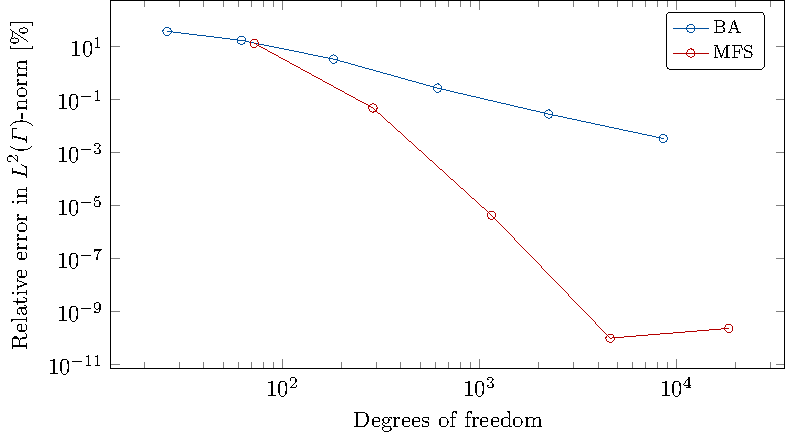
\includegraphics{Spectral}
	\caption{\textbf{Rigid scattering on a unit sphere:} A comparison between a spectral method solution (method of fundamental solution) and a finite element solution (best approximation).}
	\label{Fig:Spectral}
\end{figure}

